\newpage
\section{Autres améliorations possibles}

Une partie du stage a été de rechercher comment il serait possible de faire évoluer le travail réalisé dans Blue Banana. Les différentes pistes, que nous avons trouvé, vont donc être présentées. La première consiste à se servir des déplacements en groupe des avatars. Une présentation de ces mouvements de groupes permettra de mieux comprendre en quoi la piste d'amélioration peut être intéressante. Un mécanisme de connaissance des routes entre les Hotspots pourrait aussi être intéressant. Car actuellement les avatars se déplacent de façon aléatoire entre les Hotspots, alors que  dans les jeux vidéos les joueurs utilisent souvent les mêmes routes pour se déplacer. Cette piste permettrait de rendre les simulations et les solutions plus adaptées aux comportements des joueurs dans les MMOGs.

\subsection{Déplacements en groupes}

Les activités en groupe des avatars dans les MMOGs sont une part très importante de l'expérience que le joueur de MMOGs recherche~\cite{1501834,1255052}. Un tour d'horizon rapide des comportements sociaux des joueurs permettra de comprendre l'intérêt de cette solution. Des études ont démontré que des mouvements groupés existaient dans World of Warcraft~\cite{15141312}. La coopération et le complémentarité des joueurs d'un même groupe permettent la réussite plus facile des missions. Les groupes (guildes) sont donc de plus en plus importants, et le fonctionnement fait penser au fonctionnement d'une famille de la mafia~\cite{Jakobsson03thesopranos}.


%\newpage
\subsubsection{Étude des habitudes des joueurs de MMOG}

Plusieurs études~\cite{BreakingSteretype,1159988,1255052,StudyEQ} des comportements des joueurs mettent en avant l'importance des différentes sortes d'interactions sociales. Pour 41\% des joueurs, l'interaction sociale est l'aspect favori des MMOGS~\cite{BreakingSteretype}. Même si certaines études~\cite{1124834,1031667} expliquent que les joueurs préfèrent jouer seuls, toutes disent que les interaction sociales sont courantes, et sont un des facteurs important des MMOGs. 

\par Les liens sociaux entre les joueurs ressemblent à des interactions dans le monde \textit{réel}, avec des comportements d'adhésion que l'on peut comparer aux mariages, avec des échanges commerciaux et même des \textit{services d'église}. Des normes sociales sont aussi présentes dans le jeu en plus des règles mises en place par l'éditeur (jargons, abréviations, émoticones, etc). Dans~\cite{StudyEQ}, l'auteur a réalisé une étude sur les habitudes des joueurs de EverQuest. Il ressort de cette étude que les personnes interrogées prennent beaucoup de plaisir à avoir des relations sociales dans le jeu (3° action la plus appréciée). Lorsque les joueurs jouent en groupe, ils le font la majorité du temps avec des gens qu'il connaissent déjà (moins de 10\% avec des inconnus). Plus de 50\% des sondés sont très contents d'être dans leur guilde.


\par Dans~\cite{1124834}, les auteurs se sont intéressés aux dynamiques sociales dans les MMOG, et particulièrement dans le jeu World Of Warcraft~\cite{wow}. Une des premières observations est que les joueurs vont jouer différemment en fonction de leur niveau. Il est possible de remarquer que le temps passé en groupe évolue en fonction du niveau du joueur (voir figure~\ref{timespentgroup} ). Le pourcentage de temps passé en groupe évolue en même temps que le niveau du joueur.  
	\begin{figure}[!h]
        \centering
        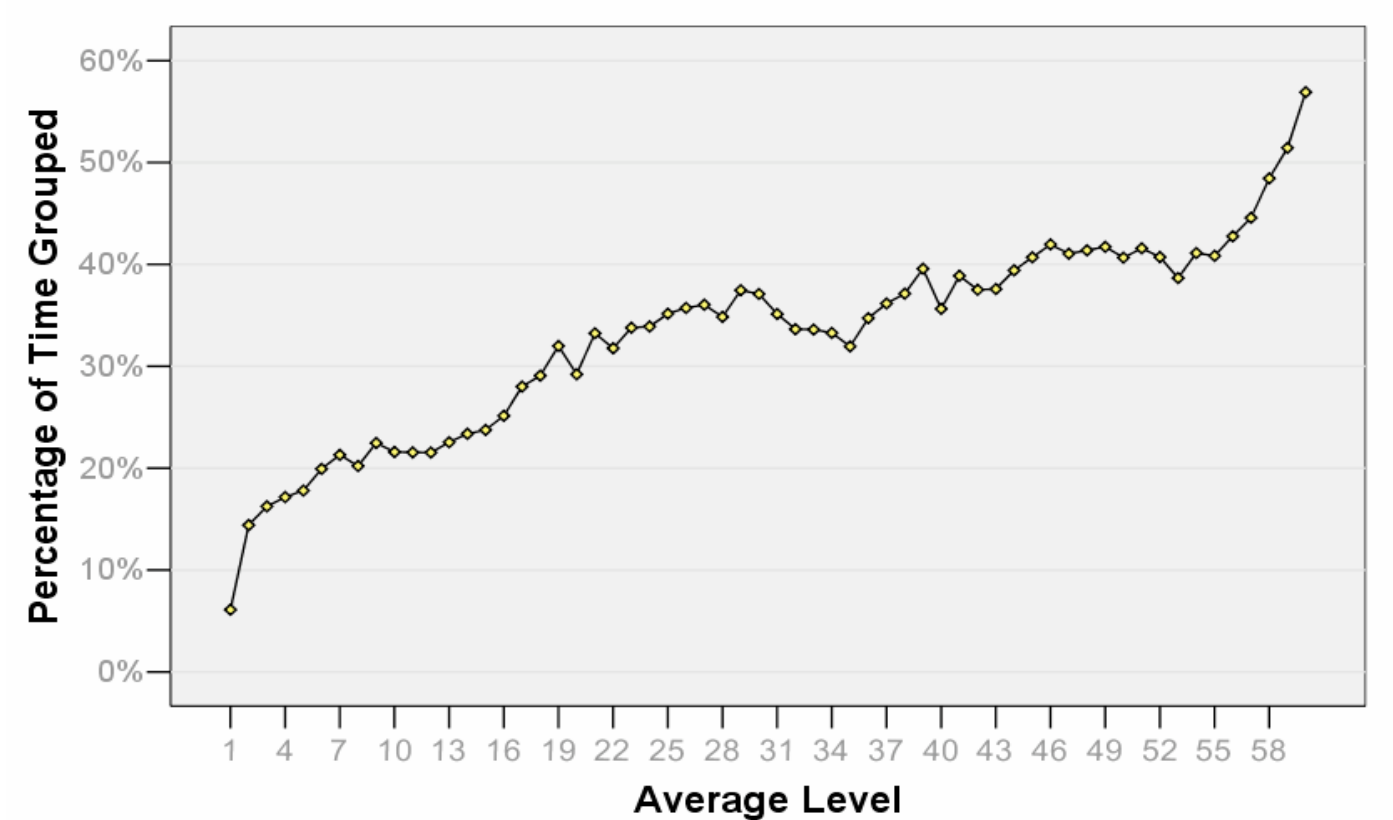
\includegraphics[scale=0.85]{./Ressources/Images/timespentgroup.png}
        \caption{Temps moyen passé en groupe, par niveau}
        \label{timespentgroup}
        \end{figure}

\par World Of Warcraft encourage les joueurs à former des groupes en utilisant deux mécanismes. Premièrement, pour qu'une complémentarité entre les habilitées des joueurs se crée. Deuxièmement, beaucoup de quêtes dans le jeu sont difficiles à réaliser tout seul. De même qu'il y a des différences de temps passé en groupe en fonction du niveau, des différences se dégagent entre le temps passé en groupe en fonction de chaque espèce se distingue aussi. Dans World Of Warcraft, 66\% des avatars appartiennent à une guilde et ce chiffre atteint 90\% si l'on tient compte des joueurs ayant au moins le niveau 43. Les joueurs appartenant à une guilde joue en moyenne plus souvent qu'un joueur sans guilde. 

\par Dans la figure~\ref{co-location}, il est possible de voir à quoi ressemble les liens entre les différents joueurs d'une même guilde de 41 membres. Tout d'abord 17 membres de la guilde n'ont jamais été observés dans la même zone qu'un autre membre. Un noyau central se distingue, il est composé de 8 joueurs qui jouent souvent ensemble, 3 autres joueurs forment un trio central où les liens épais montrent qu'ils passent beaucoup de temps ensemble. Les autres joueurs jouent avec 2 (ou moins) membres de la guilde.
	 \begin{figure}[!h]
        \centering
        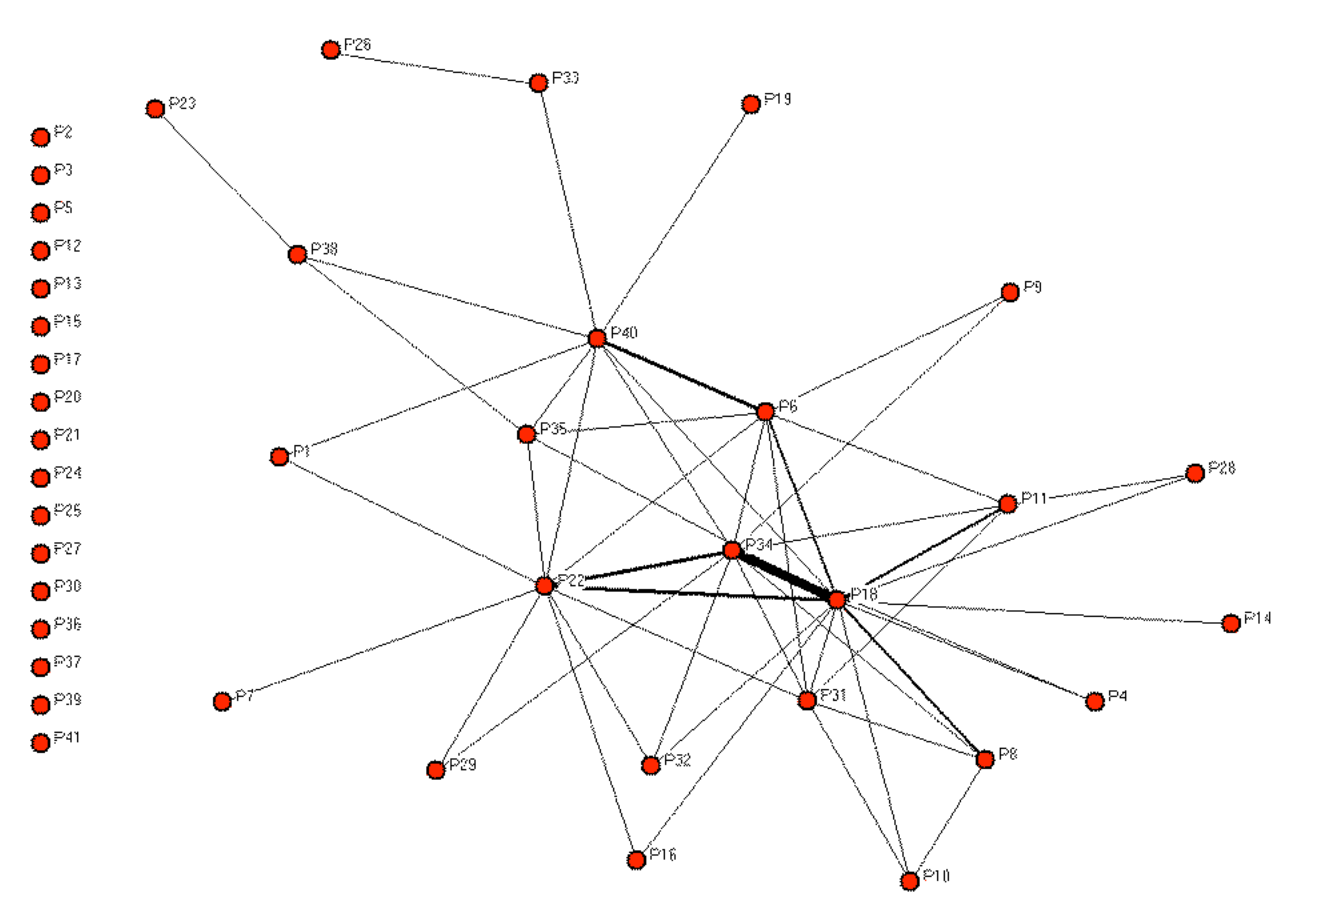
\includegraphics[scale=0.75]{./Ressources/Images/co-location.png}
        \caption{Co-location network dans une guilde de taille moyenne}
        \label{co-location}
        \end{figure}

\subsubsection{Conclusion sur l'étude des mouvements}
L'aspect communautaires des MMOGs est un des points les plus importants pour les joueurs. De plus, la majorité des études expliquent que la plupart des joueurs jouent et bougent en groupe pendant un temps non négligeable. Ces mouvements de groupe pourraient nous permettre de faire évoluer le module de rapatriement des données, en formant des groupes où seulement certaines entités feraient les différents traitements, la liste des voisins d'une entité comprendrait plusieurs éléments stables.
\par Pour mettre en place cette solution, il faudrait refaire le système de mobilité pour simuler des mouvements de groupe. Ces études sur les mouvements de groupe sont réalisées sur certains jeux~\cite{wow,everquest}, mais dans d'autres jeux ces mécanismes de groupe peuvent être moins perceptibles~\cite{sl}. Il faudrait aussi mettre en place un système d'équilibrage des requêtes lors de mouvements de groupe, sinon certains nœuds travailleront toujours pour les autres.


\subsubsection{Solution d'utilisation des mouvements de groupes}
\par L'utilisation des mouvements de groupe pourraient nous permettre de réorganiser le rapatriement des données, et ne plus considérer les nœuds indépendamment mais comme formant un groupe. Ces groupes devront avoir une organisation flexible et efficace. Les nœuds se trouvant en avant du groupe, selon la direction, pourraient être les seuls à rapatrier des données, ainsi des messages seraient économisés. Il faudrait ensuite transmettre les données vers les autres membres du groupe, plusieurs méthodes de diffusion peuvent être mises en place. La formation du groupe pourrait aussi permettre de mettre entre parenthèse la recherche de voisins pour certains nœuds. 
\par La figure~\ref{mouvgroup} montre un exemple de ce à quoi pourrait ressembler la solution. Les nœuds, en gris foncé, vont rapatrier les données qui peuvent être intéressantes. Les autres nœuds du groupe n'auront pas rapatrier les données, mais il faudra ensuite diffuser ces données vers le reste du groupe.

        \begin{figure}[!h]
        \centering
        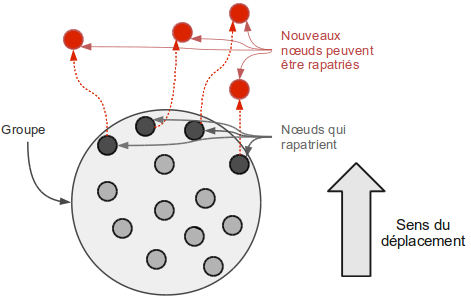
\includegraphics[scale=0.55]{./Ressources/Images/mouvgroup.png}
        \caption{Une piste pour les déplacements en groupe}
        \label{mouvgroup}
        \end{figure}

\newpage
 
\subsection{Mécanismes de connaissance des routes entre les Hotspots}
Dans cette solution, nous voudrions permettre aux avatars de suivre des routes, pour le contournement d'un obstacle par exemple. Il faudrait modifier le modèle pour ajouter des obstacles dans l'environnement. Deux solutions apparaissent rapidement pour créer ses routes. La première solution serait de définir des chemins pour contourner les obstacles, et de conserver ces chemins dans l'environnement. La deuxième solution consisterait à mettre en place un mécanisme d'apprentissage des routes par les avatars. Les avatars pourraient apprendre les routes au fur et à mesure des passages, et laisser des indications pour les avatars suivants. Cette solution permettrait de simuler un comportement réel, et ainsi d'essayer d'améliorer cette situation.
\par Les modifications sur le modèle ne seront peut être pas très simples à mettre en place. Il faudrait aléatoirement, comme il a été fait pour les Hotspots, définir des zones où les avatars ne pourraient pas passer ou seraient ralentis. Sur la figure~\ref{trajobstacle}, nous pouvons voir des trajectoires permettant d'éviter l'obstacle. Il faut définir si ces trajectoires se font par apprentissage ou si elles sont données avec l'initialisation de la carte.

	\begin{figure}[!h]
        \centering
        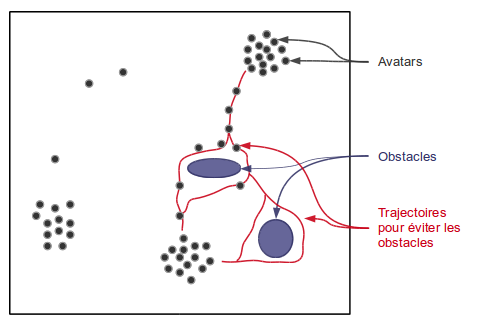
\includegraphics[scale=0.5]{./Ressources/Images/trajobstacle}
        \caption{Exemple de trajectoire d'évitement d'un obstacle}
        \label{trajobstacle}
	\end{figure}

\subsection{Conclusion sur les autres améliorations possibles}

Les différentes solutions trouvées permettraient d'étudier différents comportements prenant mieux en compte les habitudes des joueurs de MMOGs. La mise an place de ces solutions serait plus lourdes que les solutions implémentées durant le stage. 
D'autres idées d'améliorations sont aussi apparues mais sans qu'elles ne soient étudiées précisément. La possibilité de créer des liens entre des nœuds qui sont proches dans le réseau est une des idées apparues. Ainsi deux nœuds qui sont proches pourraient échanger des données rapidement et ces données pourraient servir au nœud ultérieurement ou ils pourraient les faire partager à d'autres nœuds sur le réseau virtuel. En s'inspirant du cache, les nœuds pourraient se souvenir, en fonction de la zone géographique où ils se trouvent, d'anciens nœuds déjà rencontrés et ainsi tenter de communiquer avec eux prioritairement.



